\begin{definition}[Restriction]
    Let $\mr{E} = (E,\#,\vdash)$ be an event structure.
    Let $A \subseteq E$.
    Define the restriction of $\mr{E}$ to $A$ to be
    \begin{align*}
        \mr{E} \lceil A = (A,\#_A,\vdash_A)
    \end{align*}
    where
    \begin{align*}
        X \in Con_A \iff X \subseteq A \ \wedge \ X \in Con \\
        X \vdash_A e \iff X \subseteq A \ \wedge \ e \in A \ \& \ X \vdash e
    \end{align*}
\end{definition}

\begin{definition}[Prefixing]
    Let $a$ be an event.
    For an event structure $\mr{E} = (E,\#,\vdash)$ define $a\mr{E}$ to be the event structure $(E',\#',\vdash')$ where:
    \begin{align*}
         & E' = \s{(0,a)} \cup \s{(1,e)|e \in E},                                                                                                        \\
         & \forall e_0',e_1'\in E' . e_0' \#' e_1'  \iff \exists e_0,e_1.e_0' = (1,e_0)
        \ \wedge \ e_1' = (1,e_1) \ \wedge \ e_0 \# e_1                                                                                                  \\
         & \forall X \subseteq E' . X \vdash' e' \iff e' = (0,a) \text{ or } [e' = (1,e_1) \ \wedge \ (0,a)\in X \ \wedge \ \s{e|(1,e)\in X} \vdash e_1]
    \end{align*}
\end{definition}

\subsubsection{Prefix}
\begin{definition}[Prefix]
    Let $(E,\#,\vdash,L,l)$ be a labelled event structure.
    Let $\alpha$ be a label.
    Define $\alpha(E,\#,\vdash,L,l)$ to be a labelled event structure
    $(E',\#',\vdash',L',l')$ where $(E',\#',\vdash') = \alpha(E,\#,\vdash)$
    and labels are defined as follows:
    \begin{align*}
        L' = \s{\alpha} \cup L
    \end{align*}
    and
    $$
        l'(e') = \begin{cases}
            \alpha & \text{if } e' = (0,\alpha) \\
            l(e)   & \text{if } e' = (1,e)
        \end{cases}
    $$
    for all $e' \in E'$.
\end{definition}

\subsubsection{Sum}
\begin{definition}[Sum]
    Let $\mr{E_0} = (E_0,\#_0,\vdash_0,L_0,l_0)$ and
    $\mr{E_1} = (E_1,\#_1,\vdash_1,L_1,l_1)$ be labelled event structures.
    Their sum $\mr{E_0} + \mr{E_1}$, is defined to be the structure $(E,\#,\vdash,l)$
    with events $E = \s{(0,e)|e \in E_0} \cup \s{(1,e)|e \in E_1}$,
    the disjoint union of sets $E_0$ and $E_1$,
    with injections $\iota_k: E_k \rightarrow E$, given by
    $\iota_k(e) = (k,e)$, for $k=0,1$, conflict relation
    \begin{align*}
        \forall e,e' \in E.
        e \# e' \iff & \exists e_0,e_0' \in E_0. e = \iota_0(e_0)
        \wedge e' = \iota_0(e_0') \wedge e_0 \#_0e_0'                                                      \\
                     & \text{or } \exists e_1,e_1' \in E_1. e = \iota_1(e_1) \wedge
        e' = \iota_1(e_1') \wedge e_1 \#_1 e_1'                                                            \\
                     & \text{or } \exists e_0 \in E_0,e_1 \in E_1.(e=\iota_1(e_0) \wedge e' =\iota_1(e_1)) \\
                     & \text{or } (e'=\iota_1(e_0) \wedge e =\iota_1(e_1))
    \end{align*}
    and enabling relation
    \begin{align*}
        X \vdash e \iff & X \in Con \wedge e \in E \wedge                   & \\
                        & (\exists X_0 \in Con_0,e_0 \in E_0.X = \iota_0X_0
        \wedge e = \iota_0(e_0) \wedge X_0 \vdash_0 e_0) \text{ or }          \\
                        & (\exists X_1 \in Con_1,e_1 \in E_1.X = \iota_1X_1
        \wedge e = \iota_1(e_1) \wedge X_1 \vdash_1 e_1)                      \\
    \end{align*}
    Where $Con_0,Con_1$ are defined on $\mr{E}_0$ and $\mr{E}_1$ respectively.
    We define the set of labels as $L_0 \cup L_1$ and the labelling function as:
    $$
        l(e) = \begin{cases}
            l_0(e_0) & \text{ if } e = \iota_0(e_0) \\
            l_1(e_1) & \text{ if } e = \iota_1(e_1)
        \end{cases}
    $$
\end{definition}

\subsubsection{Product}
In the product of two event structures, their events of synchronization are those pairs of events $(e_0,e_1)$, one from each event structure;
if $e_0$ is labelled $\alpha_0$ and $e_1$ is labelled $\alpha_1$ the synchronization event is
then labelled $(\alpha_0,\alpha_1)$.
Events need not synchronize however; an event in one component may not synchronize with
any event in the other.
We shall use events of the form $(e_0,*)$/$(*,e_1)$ to stand for the occurrence of an event $e_0$/$e_1$
from one component unsynchronized with any event of the other.
Such an event will be labeled by $(\alpha_0,*)$ where $\alpha_0$ is the original label of $e_0$
and * is a sort of undefined.

\begin{definition}[Product]
    Let $\mr{E_0} = (E_0,\#_0,\vdash_0,L_0,l_0)$ and
    $\mr{E_1} = (E_1,\#_1,\vdash_1,L_1,l_1)$
    be labeled event structures.
    Define their product $\mr{E_0} \times \mr{E_1}$ to be the structure $\mr{E} = (E,\#,\vdash,L,l)$
    consisting of events $E$ of the form
    \begin{align*}
        E_0 \times_* E_1 =
        \s{(e_0,*)|e_0 \in E_0}
        \cup \s{(*,e_1)|e_1 \in E_1}
        \cup \s{(e_0,e_1)| e_0 \in E_0 \wedge e_1 \in E_1}
    \end{align*}
    with projections $\pi_i : E \rightarrow_* E_i$,
    given by $\pi_i(e_0,e_1) = e_i$, for $i=0,1$, reflexive conflict relation $\doublevee$ given by
    \begin{align*}
        e \doublevee e' \iff \pi_0(e) \doublevee_0 \pi_0(e') \text{ or }
        \pi_1(e) \doublevee_1 \pi_1(e')
    \end{align*}
    for all $e,e' \in E$ we use $Con$ for the conflict-free finite sets,
    enabling relation $\vdash$ given by
    \begin{align*}
         & X \vdash e \iff X \in Con \wedge e \in E \wedge                  \\
         & (\pi_0(e)\text{ is defined } \Rightarrow \pi_0X\vdash_0\pi_0(e))
        \wedge (\pi_1(e)\text{ is defined } \Rightarrow \pi_1X\vdash_1\pi_1(e))
    \end{align*}
    Its set of labels is
    \begin{align*}
        L_0 \times_* L_1 = \s{ (\alpha_0,*)|\alpha_0 \in L_0}
        \cup \s{(*,\alpha_1)|\alpha_1 \in L_1}
        \cup \s{(\alpha_0,\alpha_1)|\alpha_0 \in L_0 \wedge \alpha_1 \in L_1}
    \end{align*}
    with projections: $\lambda_i: E \rightarrow_* E_i$ given by
    $\lambda_i(\alpha_0,\alpha_1) = \alpha_i$, for $i=0,1$.
    Its labeling function is defined to act on an event $e$ so
    \begin{align*}
        l(e) = (l_0\pi_0(e),l_1\pi_1(e))
    \end{align*}
\end{definition}

\subsubsection{Restriction}

\begin{definition}[Restriction]
    Let $\mr{E} = (E,\#,\vdash,L,l)$ be a labelled event structure.
    Let $\Lambda$ be a subset of labels.
    Define the restriction $\mr{E}\lceil \Lambda$ to be $(E',\#',\vdash',L\cap \Lambda,l')$
    where $(E',\#',\vdash')$ is the restriction of $(E,\#,\vdash)$
    to events $\s{e \in E|l(e) \in \Lambda}$ and the labeling function $l'$
    is the restriction of the original labeling function to the domain $L \cap \Lambda$.
\end{definition}

\section{Semantics of Communicating Processes}
In this section, first, we define a simple language
and we define the event structure semantics of this language.

% \subsection{Normal }

Let $\mc{A}$ be the set of possible labels for event structures.
We define a language with the following syntax:

\begin{align*}
    p ::= nil ~|~ \alpha p ~|~ p_0 + p_1 ~|~ p_0 \times p_1
    ~|~ p\lceil \Lambda
\end{align*}

where $\alpha \in \mc{A}$ and $\Lambda \subseteq \mc{A}$.

\subsection{Denotational Semantics}

\begin{definition}
    We define the semantic map $\sem{ \ }: p \ra \mathbb{E}$ where
    $\mathbb{E}$ is the set of all event structures with
    labels in $\mc{A}$ as follows:
    \begin{align*}
        \sem{nil}      & = (\emptyset,\emptyset)                  \\
        \sem{\alpha t} & = \alpha\sem{t}                        \\
        \sem{t_1 + t_2}
                        & = \sem{t_1} + \sem{t_2}                  \\
        \sem{t \lceil \Lambda}
                        & = \sem{t} \lceil \Lambda \\
        \sem{t_1 \times t_2}
                        & = \sem{t_1} \times \sem{t_2}
    \end{align*}
\end{definition}

\subsection{Examples}
In the following, we provide some examples to illustrate
how the prefix, sum, and product operators can be used to 
compose event structures.
For simplicity, assume that $ \mc{A} = \s{a,b,c}$. 

\begin{example}
    $\mr{E} = \sem{ab}$ is an event structure
    $(E,\#,\vdash,L,l)$ where:
    \begin{align*}
        E  & = \s{(0,a),(1,0,b)}                       \\
        \# & = \emptyset                               \\
           & \e \vdash (0,a), \s{(0,a)} \vdash (1,0,b) \\
        L  & = \s{a,b}                                 \\
           & l((0,a)) = a, l((1,0,b)) = b              
    \end{align*}
    The following diagram shows configurations of $\mr{E}$:
    \begin{center}
        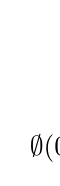
\begin{tikzpicture}[scale=0.8]
            \crd[right]{0}{0}{$\emptyset$}
            \crd[right]{0}{1}{$\s{(0,a)}$}
            \crd[right]{0}{2}{$\s{(0,a),(1,0,b)}$}
            \draw [ultra thick] (0,0) -- (0,1);
            \draw [ultra thick] (0,1) -- (0,2);
        \end{tikzpicture}
    \end{center}
\end{example}

\begin{example}
    $\mr{E} = \sem{a + b}$ is an event structure
    $(E,\#,\vdash,L,l)$ where:
    \begin{align*}
        E & = \s{(0,a),(1,b)}                \\
          & (0,a) \# (1,b)   \\
          & \e \vdash (0,a), \e \vdash (1,b) \\
        L & = \s{a,b}                        \\
          & l((0,a)) = a, l((1,b)) = b       
    \end{align*}
    The following diagram shows configurations of $\mr{E}$:
    \begin{center}
        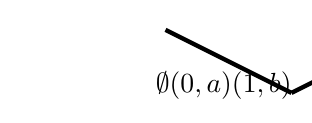
\begin{tikzpicture}[scale=0.8]
            \crd[above]{0}{0}{$\emptyset$}
            \crd[above]{-2}{1}{$\s{(0,a)}$}
            \crd[above]{2}{1}{$\s{(1,b)}$}
            \draw [ultra thick] (0,0) -- (-2,1);
            \draw [ultra thick] (0,0) -- (2,1);
        \end{tikzpicture}
    \end{center}
\end{example}


\begin{example}
    $\mr{E} = \sem{a \times b}$ is an event structure
    $(E,\#,\vdash,L,l)$ where:
    \begin{align*}
        E  & = \s{(a,*),(*,b),(a,b)}                           \\
        \# & = \e                                              \\
           & \e \vdash (a,*), \e \vdash (*,b),\e \vdash (a,b)  \\
        L  & = \s{(a,*),(*,b),(a,b)}                           \\
           & l((a,*)) = (a,*), l((*,b)) = (*,b),l((a,b))=(a,b) 
    \end{align*}
    The following diagram shows configurations of $\mr{E}$:
    \begin{center}
        \begin{tikzpicture}[scale=0.8]
            \crd[above]{0}{0}{$\emptyset$}
            \crd[left]{-2}{1}{$\s{(a,*)}$}
            \crd[right]{2}{1}{$\s{(*,b)}$}
            \crd[above]{0}{2}{$\s{(a,*),(*,b)}$}
            \crd[above]{2}{3}{$\s{(a,b)}$}
            \draw [ultra thick] (0,0) -- (-2,1);
            \draw [ultra thick] (0,0) -- (2,1);
            \draw [ultra thick] (2,1) -- (0,2);
            \draw [ultra thick] (-2,1) -- (0,2);
            \draw [ultra thick] (0,0) -- (2,3);
        \end{tikzpicture}
    \end{center}
\end{example}

In \cite{hp} there is no formal definition of the actual cause
in extended causal models.
So, here we provide a new definition of the actual cause
in the context of extended causal models.


\begin{definition}
    $\vec X = \vec x$ is an actual cause of $\varphi$ in $(M,\vec u)$ if the following three conditions hold:
    \begin{itemize}
        \item  \textbf{AC1.} $(M,\vec u)\models (\vec X = \vec x) \wedge \varphi \wedge $.
        \item  \textbf{AC2. }There exists a partition $(\vec Z, \vec W)$ of $\mathcal{V}$ with $\vec X \subseteq \vec Z$ and some setting $(\vec x',\vec w')$ of the variables in $(\vec X,\vec W)$ such that if $(M,\vec u)\models \vec Z = z^*$ for all $Z\in \vec Z$, then both of the following conditions hold:

              (a) $(M,\vec u)\models[\vec X \leftarrow \vec x', \vec W \leftarrow \vec w']\neg \varphi
                  \wedge \vec V = \vec v
                  \wedge  \vec v \in \mathcal{E}$.

              (b) $(M,\vec u)\models[\vec X\leftarrow \vec x, \vec W'
                      \leftarrow \vec w', \vec Z'\leftarrow \vec z^*]
                  \vec V = \vec v \wedge (\vec v \in \mc{E} \Rightarrow \varphi)$
              for all subsets $Z'$ of $\vec Z$.

        \item  \textbf{AC3.} $\vec X$ is minimal; no subset of $\vec X$ satisfies conditions $AC1$ and $AC2$.
    \end{itemize}
    Where $\vec v$ is the value of endogenous variables.
\end{definition}

Let $\mathbb{E}$ be the all triples of the form
$(E,\#',\vdash')$ on the set of events $E$ where
$\#' \subseteq E \times E$ and
$\vdash' \subseteq \mc{P}(E) \times E$.
We define a function
$ES: \times_{V \in \mc{V}\setminus \s{PV}} \mc{R}(V) \rightarrow \mathbb{E}$ which intuitively returns the event structure
that can be derived from the values of the endogenous variables
in the model excluding $PV$.
Let $\vec v$ be a vector of the values of the variables
in $\mc{V} \setminus \s{PV}$ and $\vec v(V)$ be the value of
$V$ in $\vec v$ for each $V \in \mc{V} \setminus \s{PV}$.
We define the function $ES$ so that if
$ES(\vec v) = (E,\#',\vdash')$ we have:
\begin{align*}
    \forall e,e' \in E. e \#' e' & \iff \vec{v}(C_{e,e'}) = \T \\
    \forall s \in \mathcal{P}(E), e \in E.  s \vdash' e
                                 & \iff \vec{v}(EN_{s,e}) = \T
\end{align*}
We define $\mathcal{E}$, the set of all allowable
settings of the endogenous variables, to be the vector of
values such as $\vec v'$ for which $ES(\vec v)$ is an
event structure.

Finally, to encode the property violation,
we define the function of $PV$ such that
if the value of the endogenous variables is
$\vec v$ then we have:
\begin{align*}
    PV = \T \iff S \cap \mc{F}(ES(\vec v)) = \e
\end{align*}

\subsection{Actual Cause of Unsafe Behavior}

Using the definition of the actual cause in the extended causal
model, we can rewrite the definition for unsafe behaviors in
event structures as follows:

\begin{definition}
    Let $\mr{E} = (E,\#,\vdash)$ be an event structure and
    $\mc{M}$ be the causal model of an unsafe behavior in
    $\mr{E}$ where unsafe behavior is specified as the
    function $F_{PV}$ in $\mc{M}$.
    We say $\vec X = \vec x$ is an actual cause of
    the unsafe behavior in $\mr{E}$ if the following
    conditions hold:
    \begin{itemize}
        \item  \textbf{AC1.} $M\models \vec X = \vec x
                  \wedge PV = \T$
        \item  \textbf{AC2. }There exists a partition $(\vec Z, \vec W)$ of $\mathcal{V}$ with $\vec X \subseteq \vec Z$ and some setting $(\vec x',\vec w')$ of the variables in $(\vec X,\vec W)$ such that if $(M,\vec u)\models \vec Z = z^*$ for all $Z\in \vec Z$, then both of the following conditions hold:

              (a) $M \models[\vec X \leftarrow \vec x', \vec W \leftarrow \vec w']
                  PV = \F
                  \wedge \vec V = \vec v
                  \wedge  \vec v \in \mathcal{E}$.

              (b) $M \models[\vec X\leftarrow \vec x, \vec W' \leftarrow \vec w', \vec Z'\leftarrow \vec z^*]
                  \vec V = \vec v
                  \wedge
                  (\vec v \in \mathcal{E} \Rightarrow PV = \T)
              $
              for all subsets $Z'$ of $\vec Z$.

        \item  \textbf{AC3.} $\vec X$ is minimal; no subset of $\vec X$ satisfies conditions $AC1$ and $AC2$.
    \end{itemize}
    Where $\vec v$ is the value of endogenous variables.
\end{definition}

We define the following programs:
\begin{align*}
    N & = p_i q_i f_{ad} + q_i p_i f_{ad} \\
    C & = p_o \times q_o \\
    SDN & = (N \times C)\lceil \Lambda \\
    \Lambda & = \s{(p_i,p_o),(q_i,q_o),(f_{ad},*)}
\end{align*}
This program captures the update behavior of the network 
figure \ref{fig:blacklist}.
Assume that two updates, $p$ and $q$ happening in the network.
$p$ replaces the path $ab$ with $ac$ and $q$ replaces
the path $cb$ with $cd$.
Let $C$ be the controller that concurrently sends commands for these
updates, $p_o,q_o$.
We use $p_i$ and $q_i$ for actions of receiving these commands and
$f_{ad}$ for the action of forwarding a packet from $a$ to $d$.
For simplicity, we do not consider any forwarding in the network 
other than $f_{ad}$.
Event structure of the $SDN$ has the configurations as depicted 
in figure \ref{fig:blacklist:es}.
Blacklisted nodes are nodes in the network that must not
be reachable \cite{network-abstractions}.
Let's assume the network in figure \ref{fig:blacklist} as
an example where the node $d$ is blacklisted.
For simplicity we assume that we require
$d$ not reachable only from $a$.
Thus, we consider the existence of configurations
$\s{p_1,q_1,ad_1}$ and $\s{p_2,q_2,ad_2}$ in an event structure
as a property violation.
In this example we can prove that $C_{p_1,q_1} = \F$ is an 
actual cause of the property violation.